\documentclass[12pt]{article}

\usepackage{tikz}
\usetikzlibrary{automata, positioning}
\begin{document}
	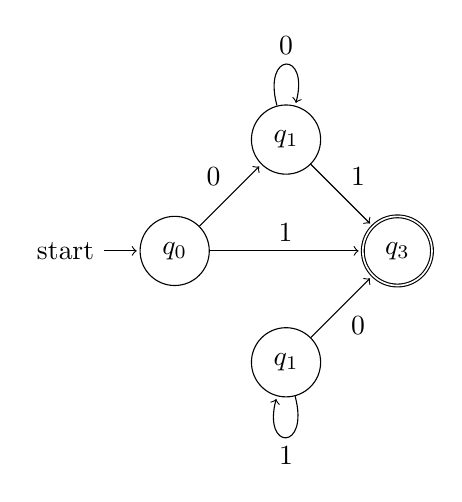
\begin{tikzpicture}[shorten >= 1pt, node distance=2cm, on grid, auto]
	\node[state, initial] (q_0) {$q_0$};
	\node [state] (q_1) [above right=of q_0] {$q_1$};
	\node [state] (q_2) [below right=of q_0] {$q_1$};
	\node [state, accepting] (q_3) [below right=of q_1] {$q_3$}; 
	\path [->]
	(q_0) edge  node {0} (q_1) 
	      edge  node {1} (q_3)
    (q_1) edge  node  {1} (q_3)
          edge [loop above] node {0} ()
    (q_2) edge  node [swap] {0} (q_3) 
          edge [loop below] node {1} ();
		  
	\end{tikzpicture}
\end{document}